\section{Semantic Segmentation}

\todo[inline, color=red!50]{Add topic: Metrics (accuracy etc.)}

Identify pixels in images belonging to a specific class, sometimes additionally identifying pixels to belong to a specific instance of a class.
It can thus be understood as supervised learning at the pixel level.
\begin{center}
	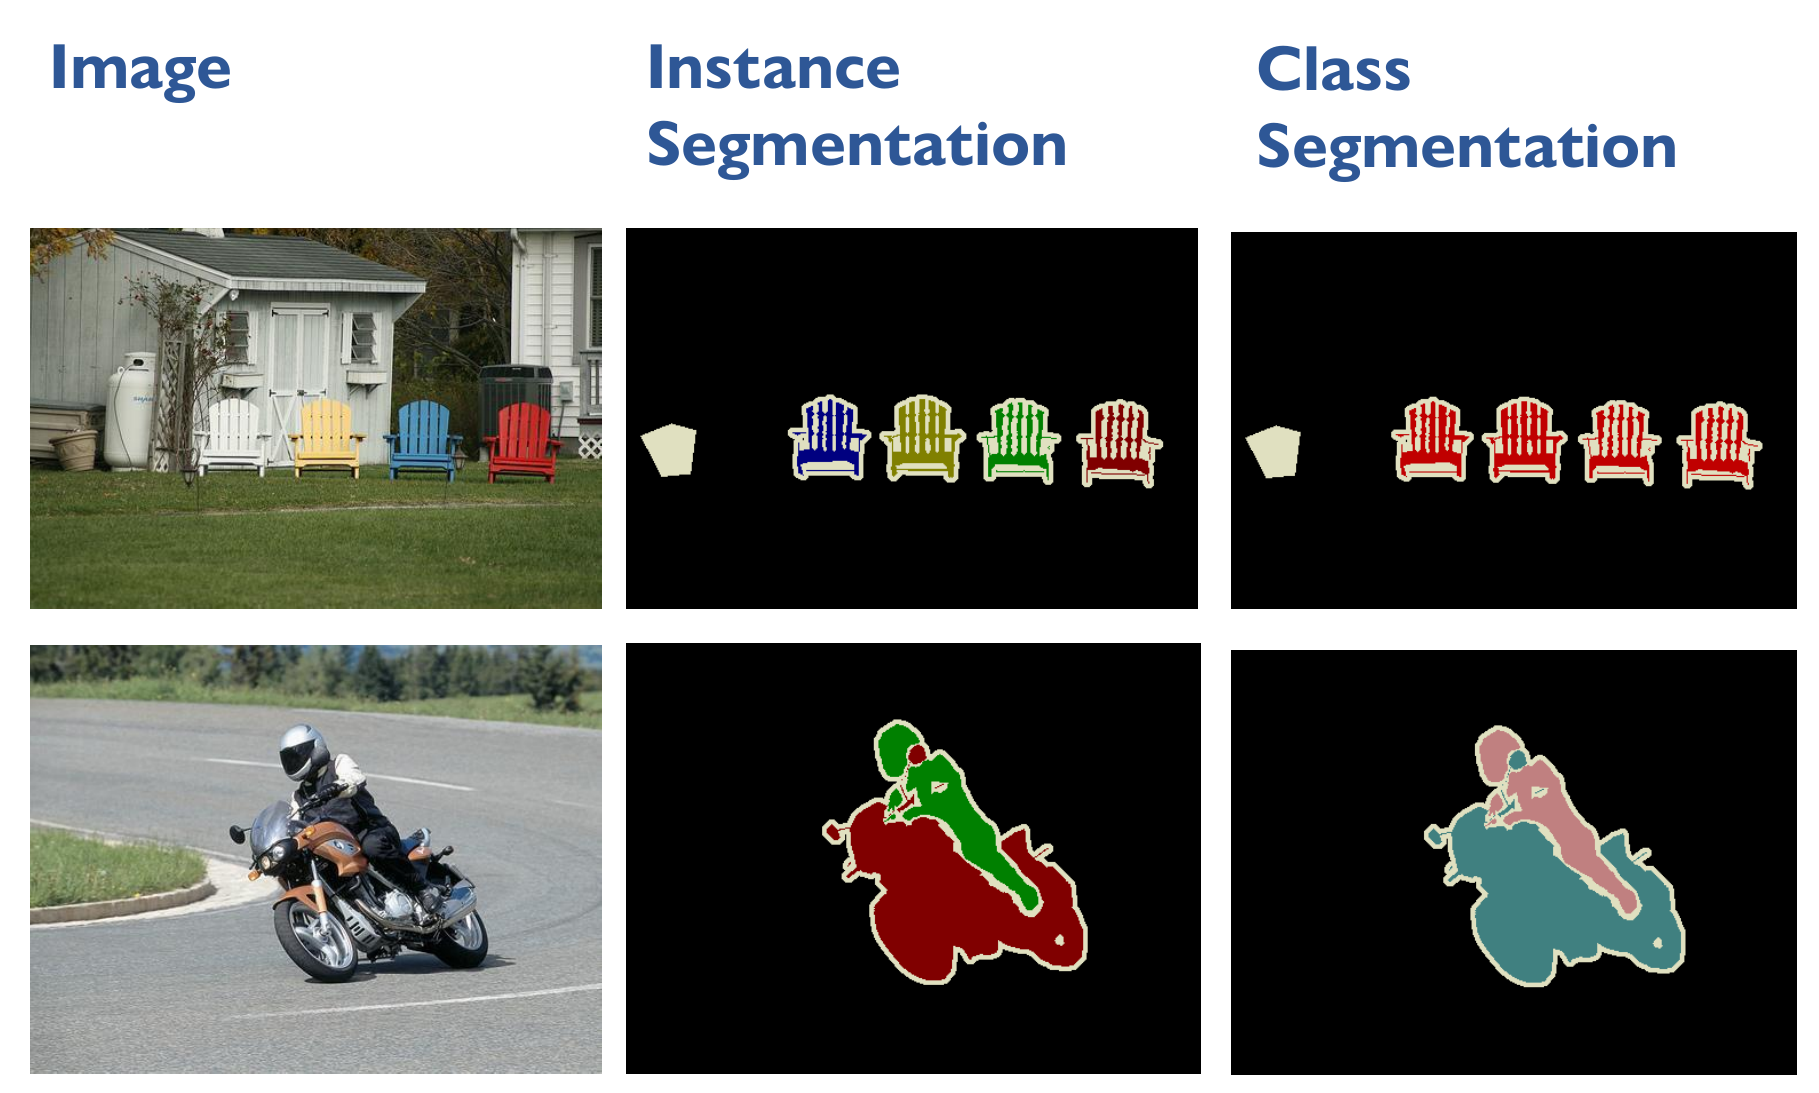
\includegraphics[width=0.7\linewidth]{img/semantic_segmentation}
\end{center}
Non-semantic segmentation tries to find regions in images without any additional information like classes or similar.
It is thus similar to unsupervised learning and often a bottom-up approach.
Segmentation in general tries to find a compact representation of a scene in terms of regions which share common properties.

\subsection{k-Means Clustering}
Is not an optimal solution to cluster an image. Lloyds algorithm is one possibility to do clustering
\begin{enumerate}
	\item[-\ ] Initialise cluster centers (for example randomly)
	\item Calculate which samples belong to which clusters
	\item Calculate mean values of clusters as new centres
	\item[-\ ] Iterate until clusters don't change
\end{enumerate}
Problems:
\begin{itemize}
	\item Number of clusters must be given
	\item Cluster shapes are given (spherical)
\end{itemize}

\subsection{Mean Shift Clustering}
The shape of the clusters should be variable and not be determined by the method. Mean shift clustering can be achieved by the algorithm
\begin{enumerate}
	\item Search for the maximum of the feature densitity from a given position in the image
	\item Define cluster as the set of positions that converge to the same maximum
\end{enumerate}
The problem to search for local maxima of the features without having a feature distribution available directly.
The solution is to use a Kernel Density Estimation to describe the distribution, for example using the Gaussian kernel.
Or using the Derivative of the Gaussian to get an approximation directly.
\begin{align*}
	\hat{f}_h(x) &= \frac{1}{nh}\sum_{i=1}^{n}K\left(\frac{x-x_i}{h}\right)\\
	K\left(\frac{x-x_i}{h}\right) &= \frac{1}{\sqrt{2\pi}} e^{-\frac{(x-x_i)^2}{2h^2}}
\end{align*}
\begin{center}
	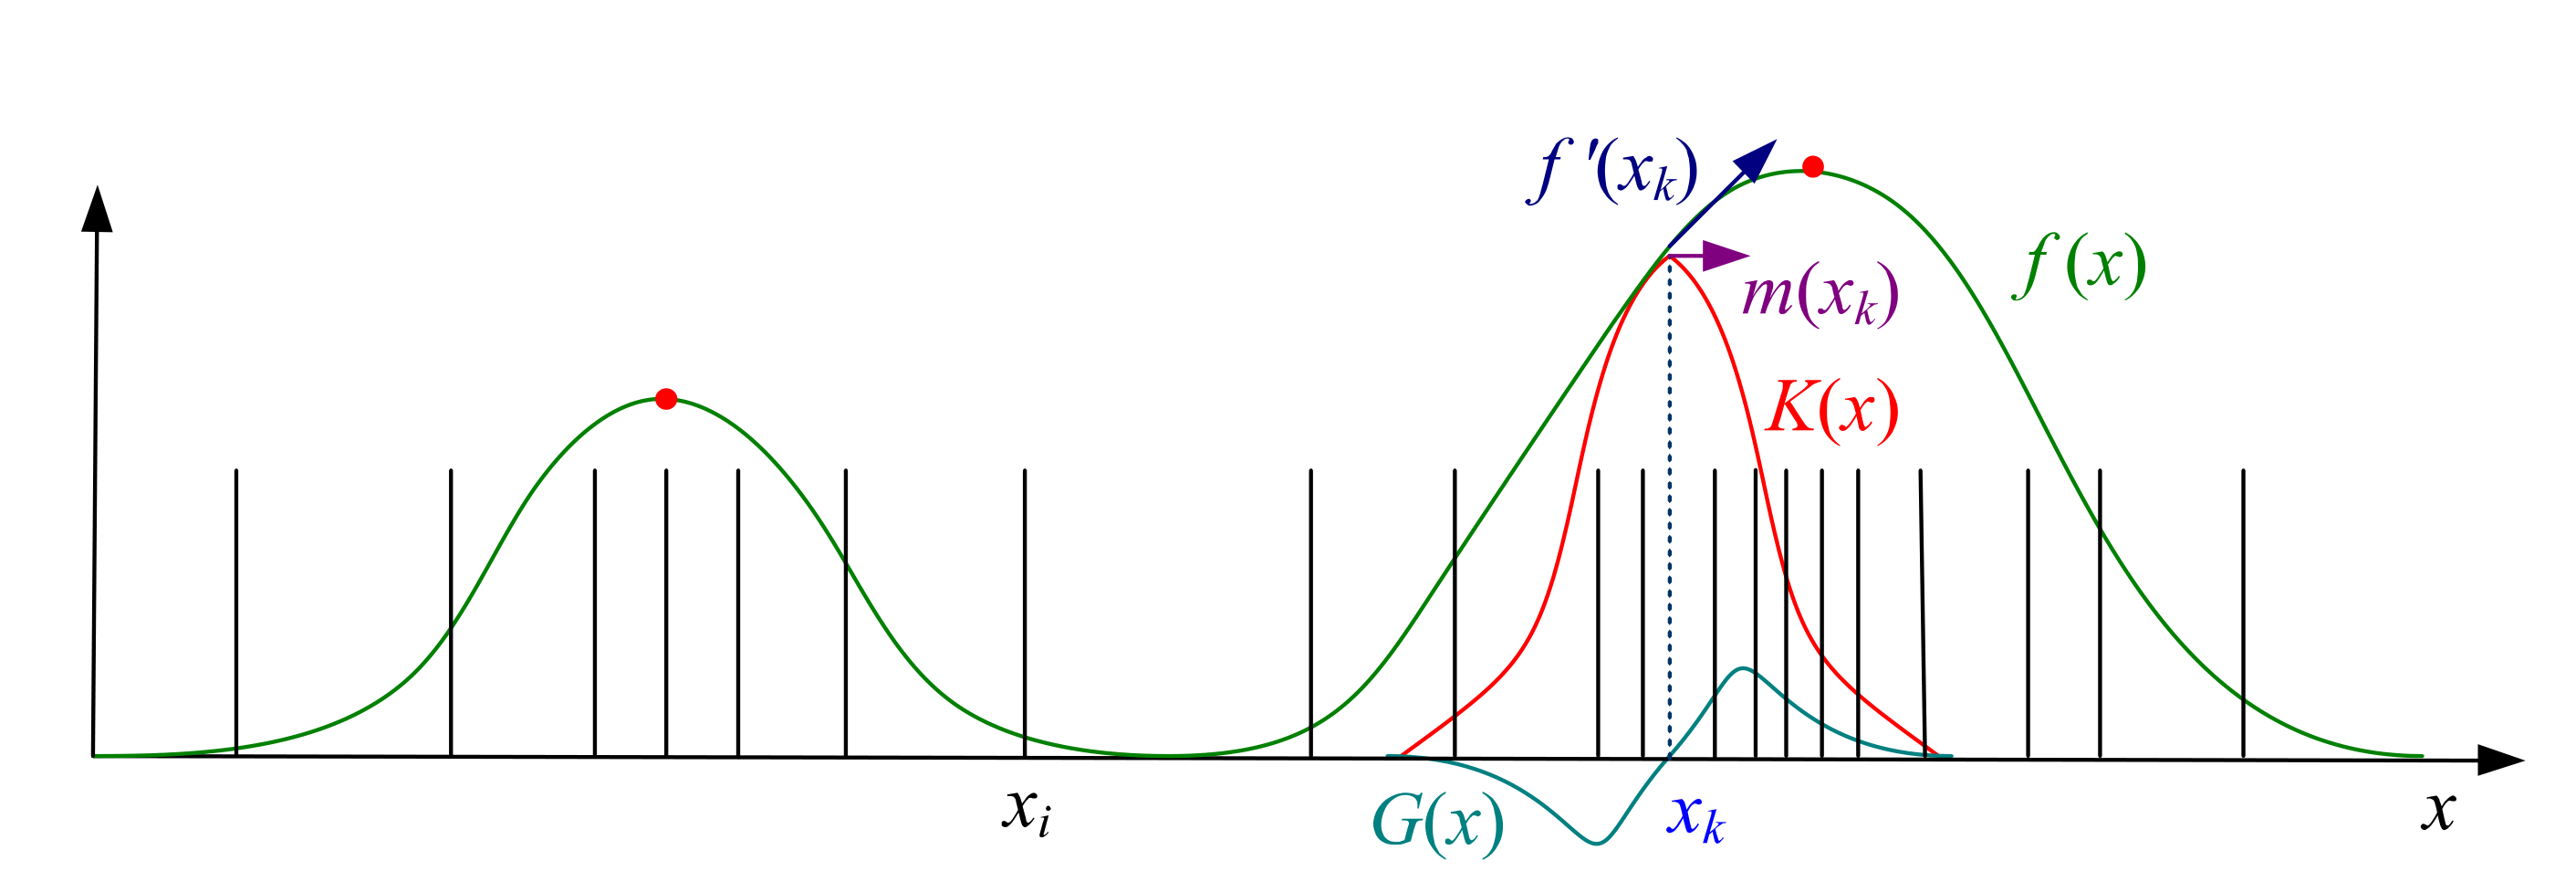
\includegraphics[width=0.7\linewidth]{img/kernel_density_estimation}
\end{center}

\subsubsection{Mean Shift Algorithm}
\begin{itemize}[label=-]
	\item[] For all positions $x$ in the image
	\item Calculate the mean $\samplemean{x}$ in the environment $N(x)$
	\begin{equation*}
		\samplemean{x} = \frac{\sum_{x_i \in N(x)} K(x_i - x) x_i }{\sum_{x_i \in N(x)} K(x_i - x)}
	\end{equation*}
	\item Set $x$ to the mean $\samplemean{x}$
	\item Iterate until $x$ does not change
\end{itemize}
\textbf{Attraction basins} are regions from which all trajectories lead to the same node.
\begin{center}
	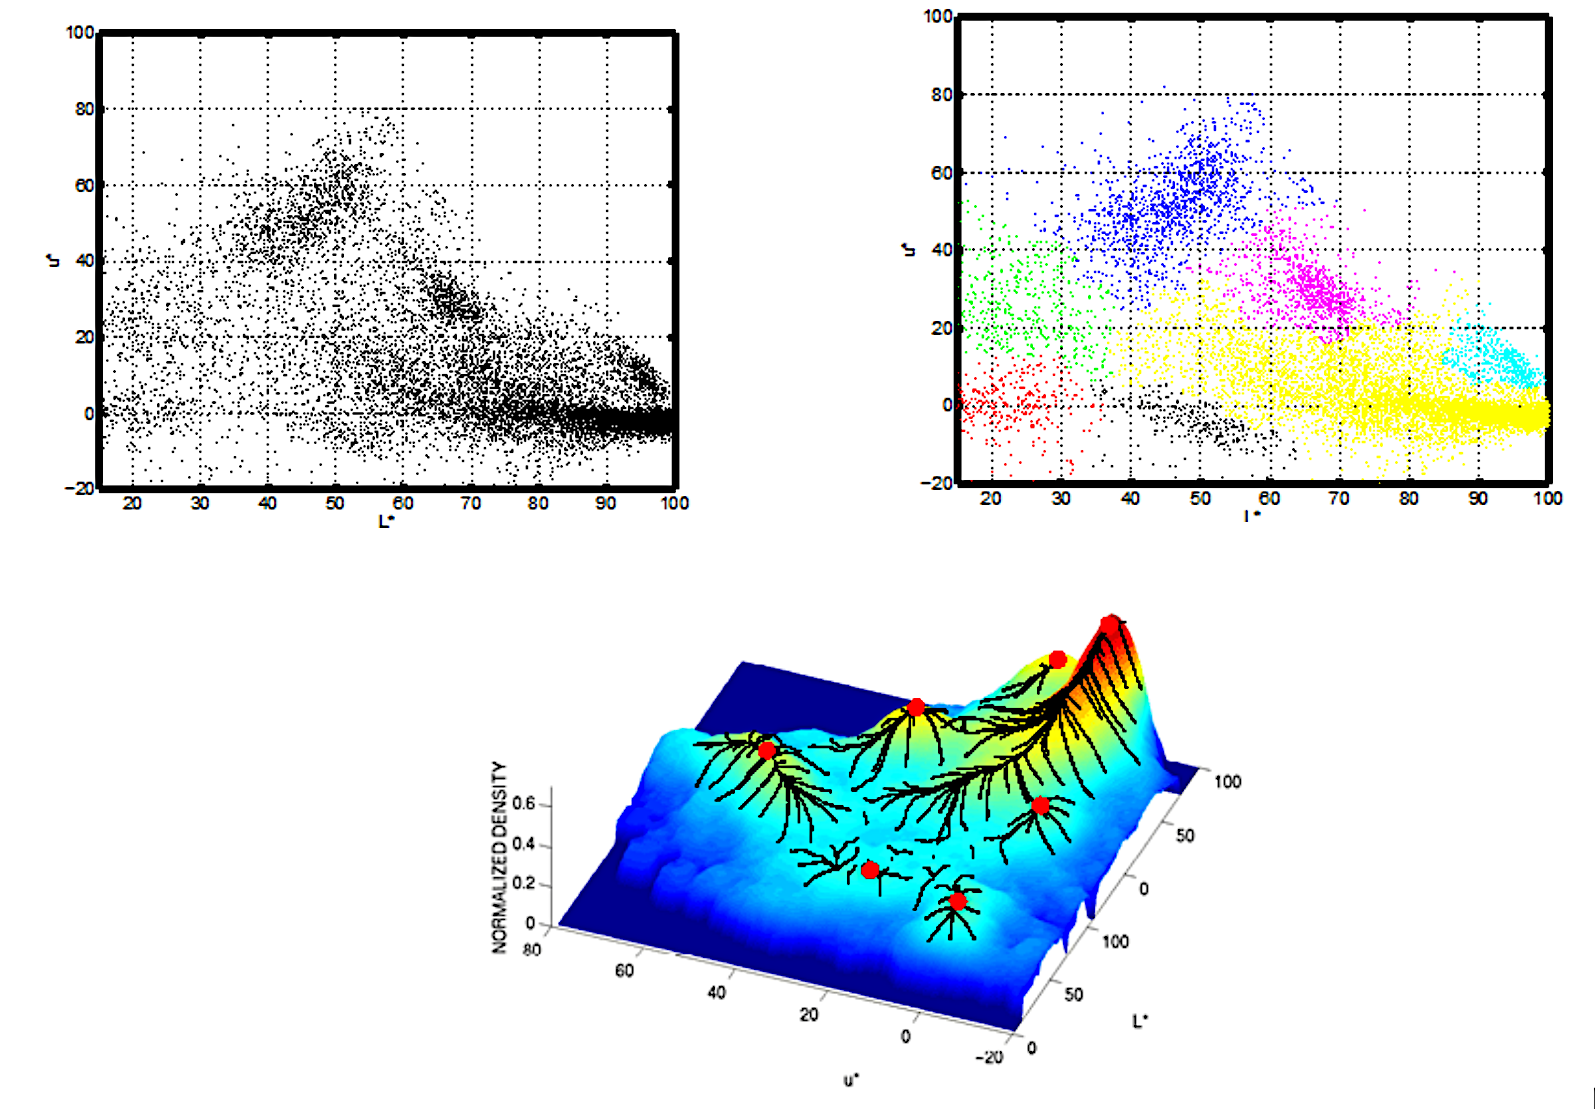
\includegraphics[width=0.7\linewidth]{img/attraction_basins}
\end{center}

\subsection{Segmentation by Graph Cuts}
Images are seen as graph with a node for every pixel with edges between nodes with an affinity weight for each edge.
This weight  measures similarity, for example inversely proportional to difference in colour and position.
\begin{definition}
	Let $G=(V,E)$ be a graph. Each edge $(u,v)$ has a weight $w(u,v)$ that represents the similarity between $u$ and $v$.
	Cut $G$ into two disjoint graphs with node sets $A$ and $B$ by removing all edges between those sets. Assign a value to the cut as follows
	\begin{equation*}
		\text{cut}(A,B) = \sum_{u\in A,v\in B}^{w(u,v)}
	\end{equation*}
\end{definition}
Minimal value cuts often cuts too small groups. A better approach is to use normalised cuts:
\begin{align*}
	\text{Ncut}(A,B) &= \frac{\text{cut}(A,B)}{\text{assoc}(A,V)} + \frac{\text{cut}(A,B)}{\text{assoc}(B,V)}\\
	\text{assoc}(A,V) &= \sum_{u\in A, t\in V}^{w(u,t)}
\end{align*}
where $V$ is the set of all vertices.

\subsection{Superpixels}
The problem is that images contain many pixels and it is thus inefficient for graph calculations.
The solution is to calculate \emph{superpixels} by grouping similar pixels first.
This is cheap but leads to over-segmentation. As soon as the superpixels are calculated, normalised graph cuts can be applied.

\subsection{Features}
Usually, Raw Input pixel values are not used as input features, as this makes the input space too big.
Instead a feature vector is calculated for each pixel or set of pixels.
These feature calculate certain properties of an image or image region.
Besides classification tasks, these vectors are also used to find subregion or image stitching, and more.

\subsubsection{Feature Properties}
Features should be invariant to
\begin{itemize}[label=-]
	\item Translation
	\item Rotation
	\item Scaling
	\item Illumination, colour changes
	\item Transformation (Skewing)
\end{itemize}

\subsubsection{Filter Banks}
\begin{center}
	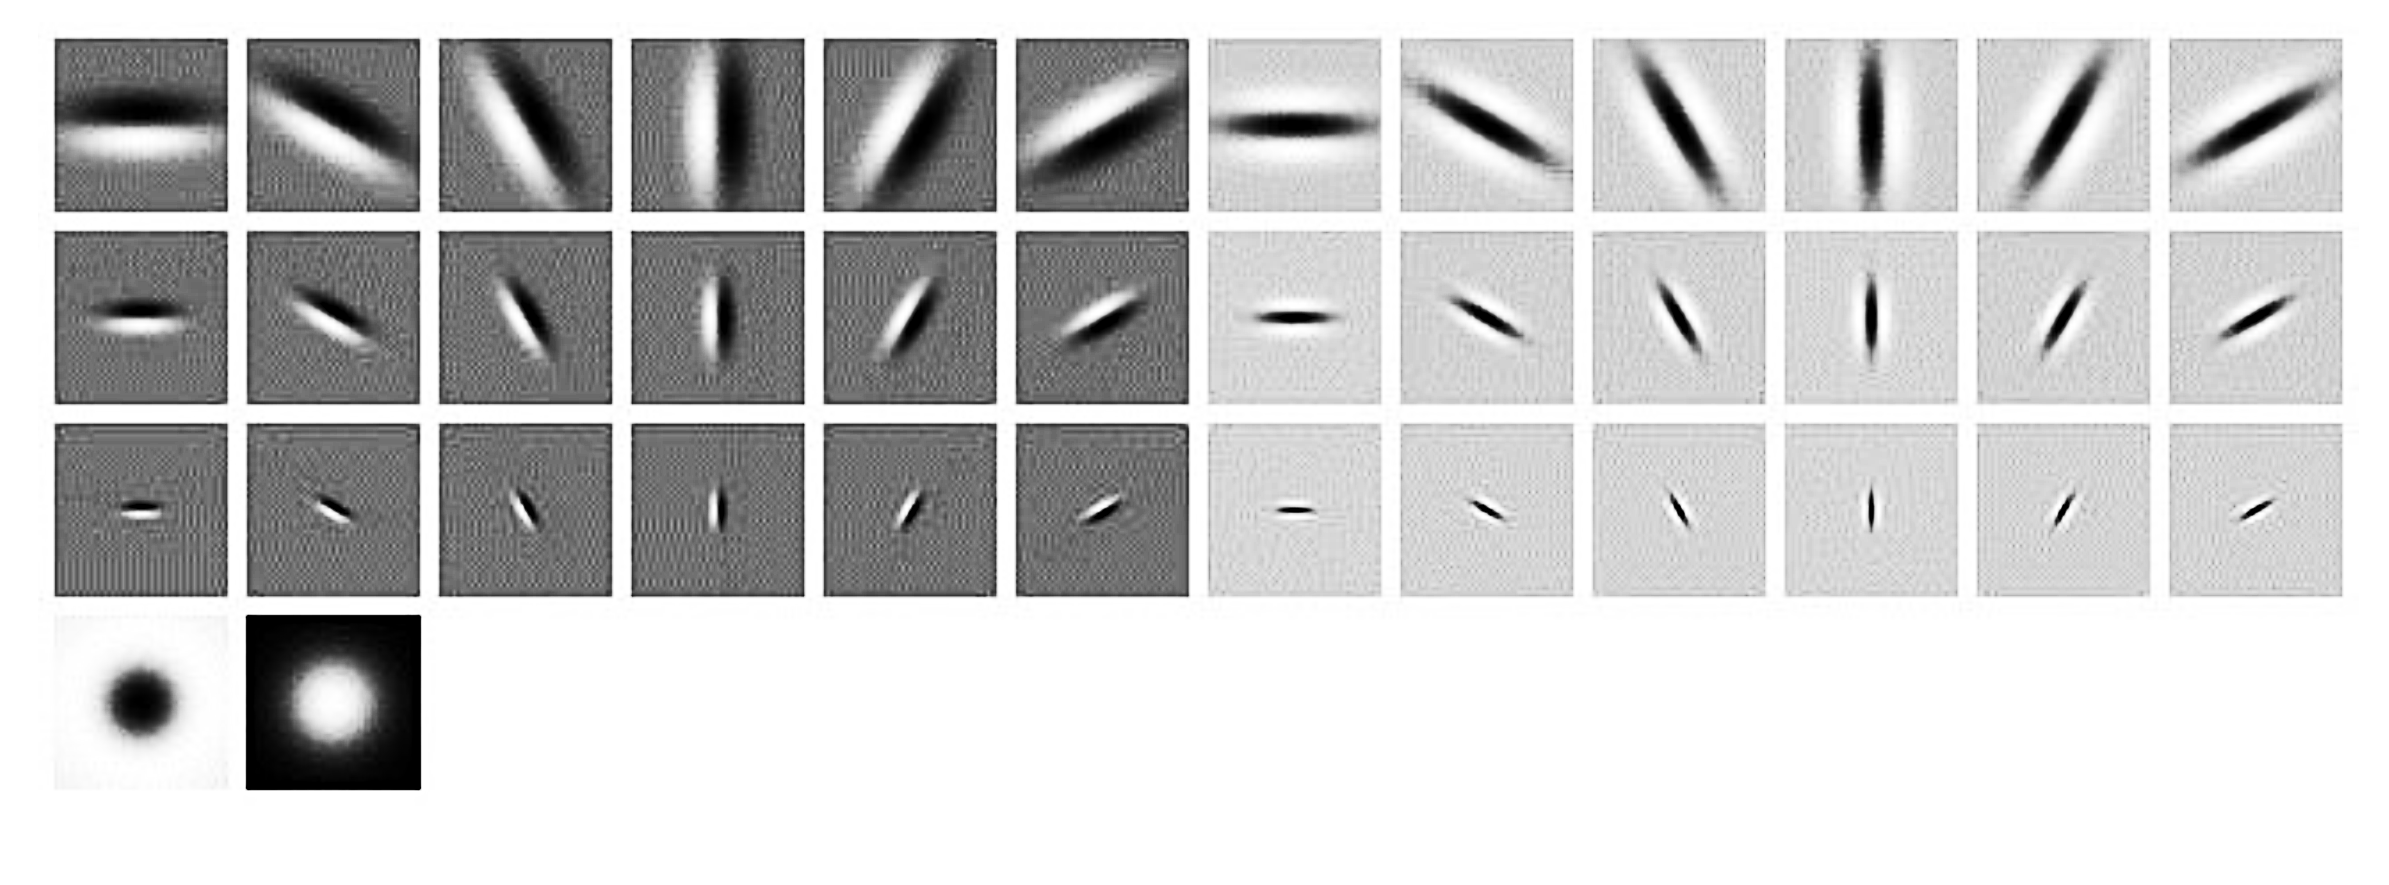
\includegraphics[width=0.6\linewidth]{img/filter_bank}
\end{center}
\begin{itemize}
	\item RFS Filters: edge and line filters at six orientations and three scales, Gaussian and Laplacian of Gaussian
	\item MR8 Filters: Maxima of RFS Filters at each scale
\end{itemize}

\subsubsection{Texture Characteristics}
Textons use the texture descriptor as vectors of filter bank outputs. Textons found by clustering are called a dictionary generation.
For comparison, use the similarity between regions in the Texton histograms directly.

\subsubsection{Grey Level Co-occurence Matrices (GLCMs)}
Measurement of how often a specific combination of a colour value between a pixel and its neighbours occur.
This results in a $256\times 256$ matrix for the 256 grey values.
Additional features like entropy, energy, homogeneity, contrast or dissimilarity can be calculated from the matrix.

\subsubsection{Scale Invariant Feature Transform (SIFT)}
Popular feature descriptor for various tasks such as object matching, image stitching and more.
It is a combination of detector and descriptor. The descriptor uses the histogram of the gradient.
SIFT results in a 128-dimensional vector.
\begin{center}
	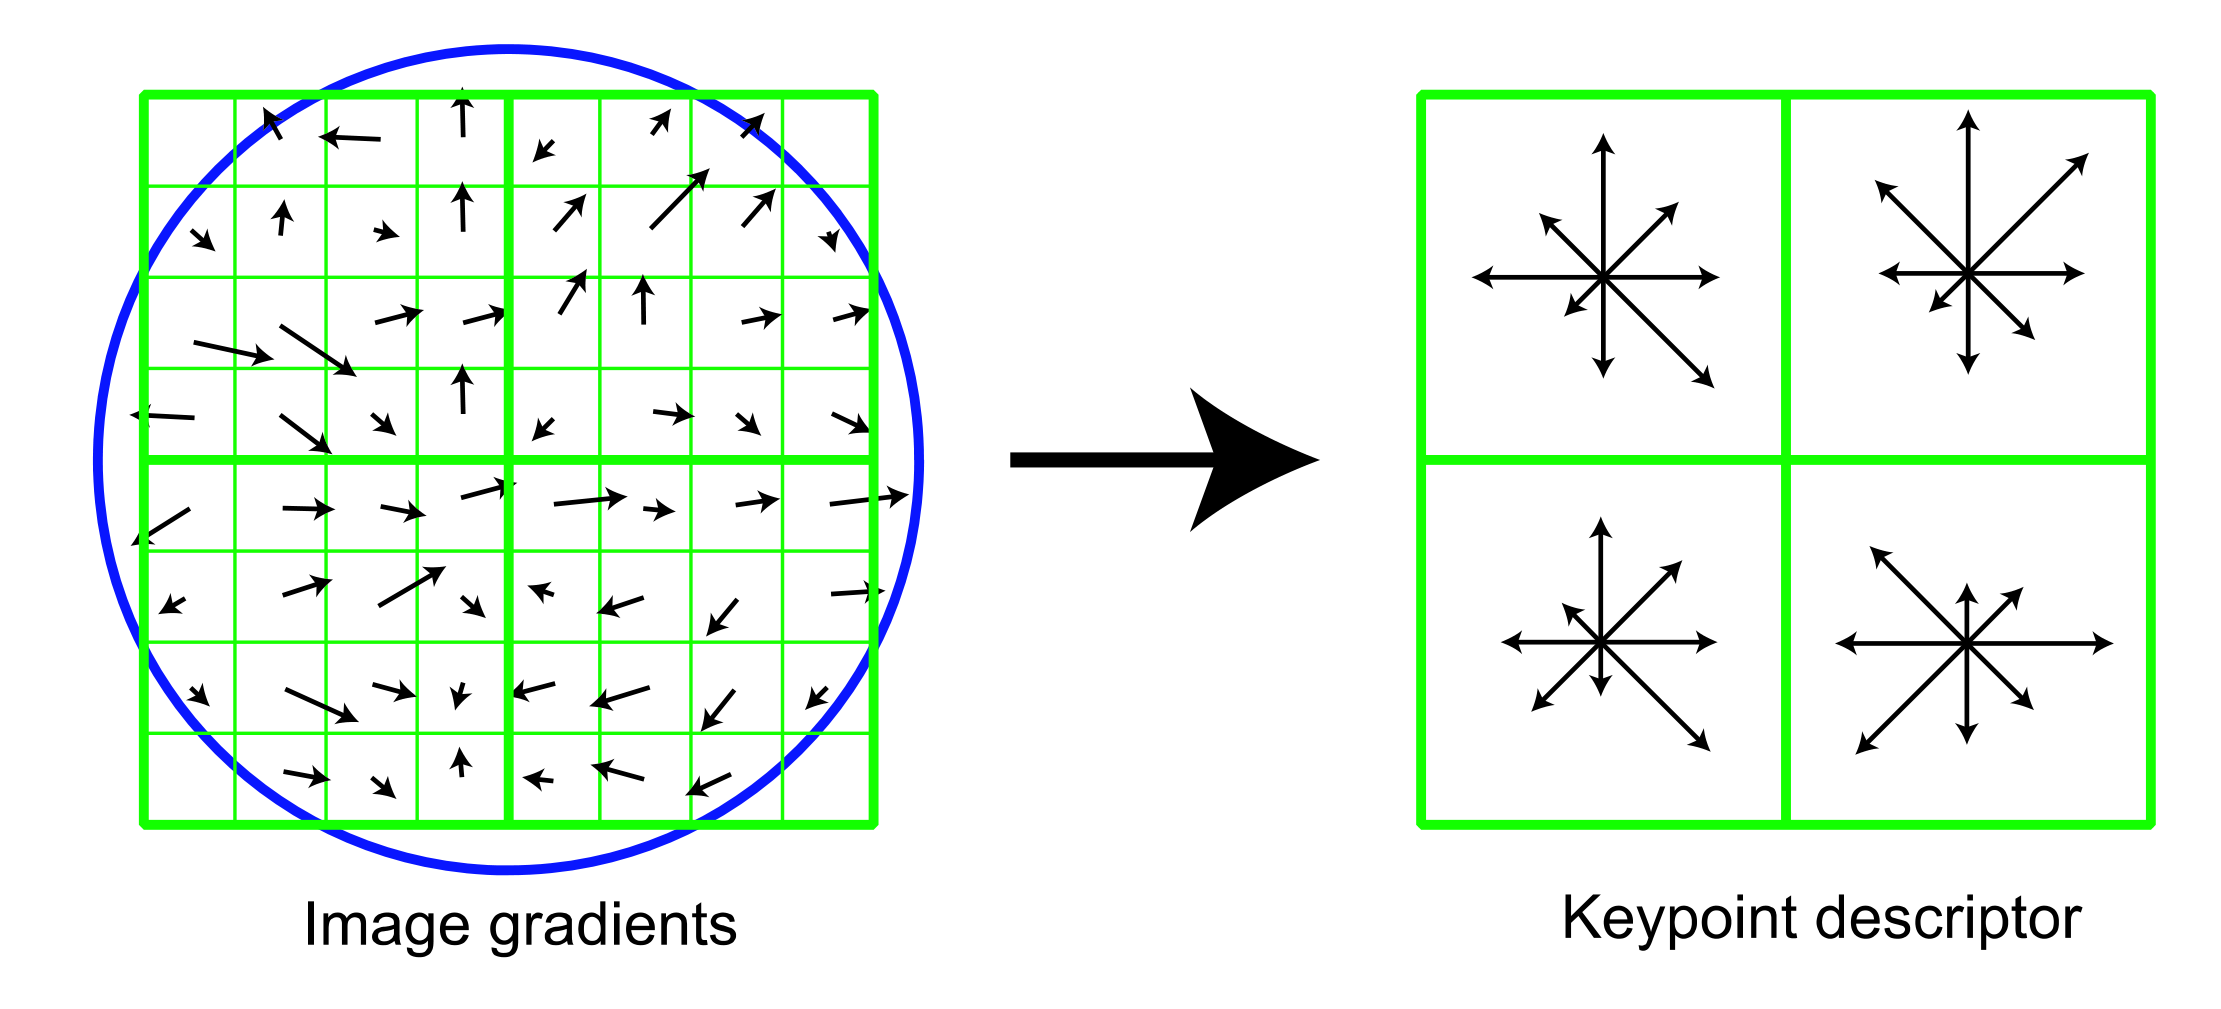
\includegraphics[width=0.6\linewidth]{img/SIFT}
\end{center}

\subsubsection{Histogram of Oriented Gradients (HOG)}
Computes the gradient images in x and y, and divides the image into cells.
Compute histogram of gradient orientation in cell, normalise and flatten it into a feature vector.

\subsubsection{HOGles}
"Invert" the HOG features to simulate the image that generates it. This is a helpful tool to understand bad detections.

\begin{center}
	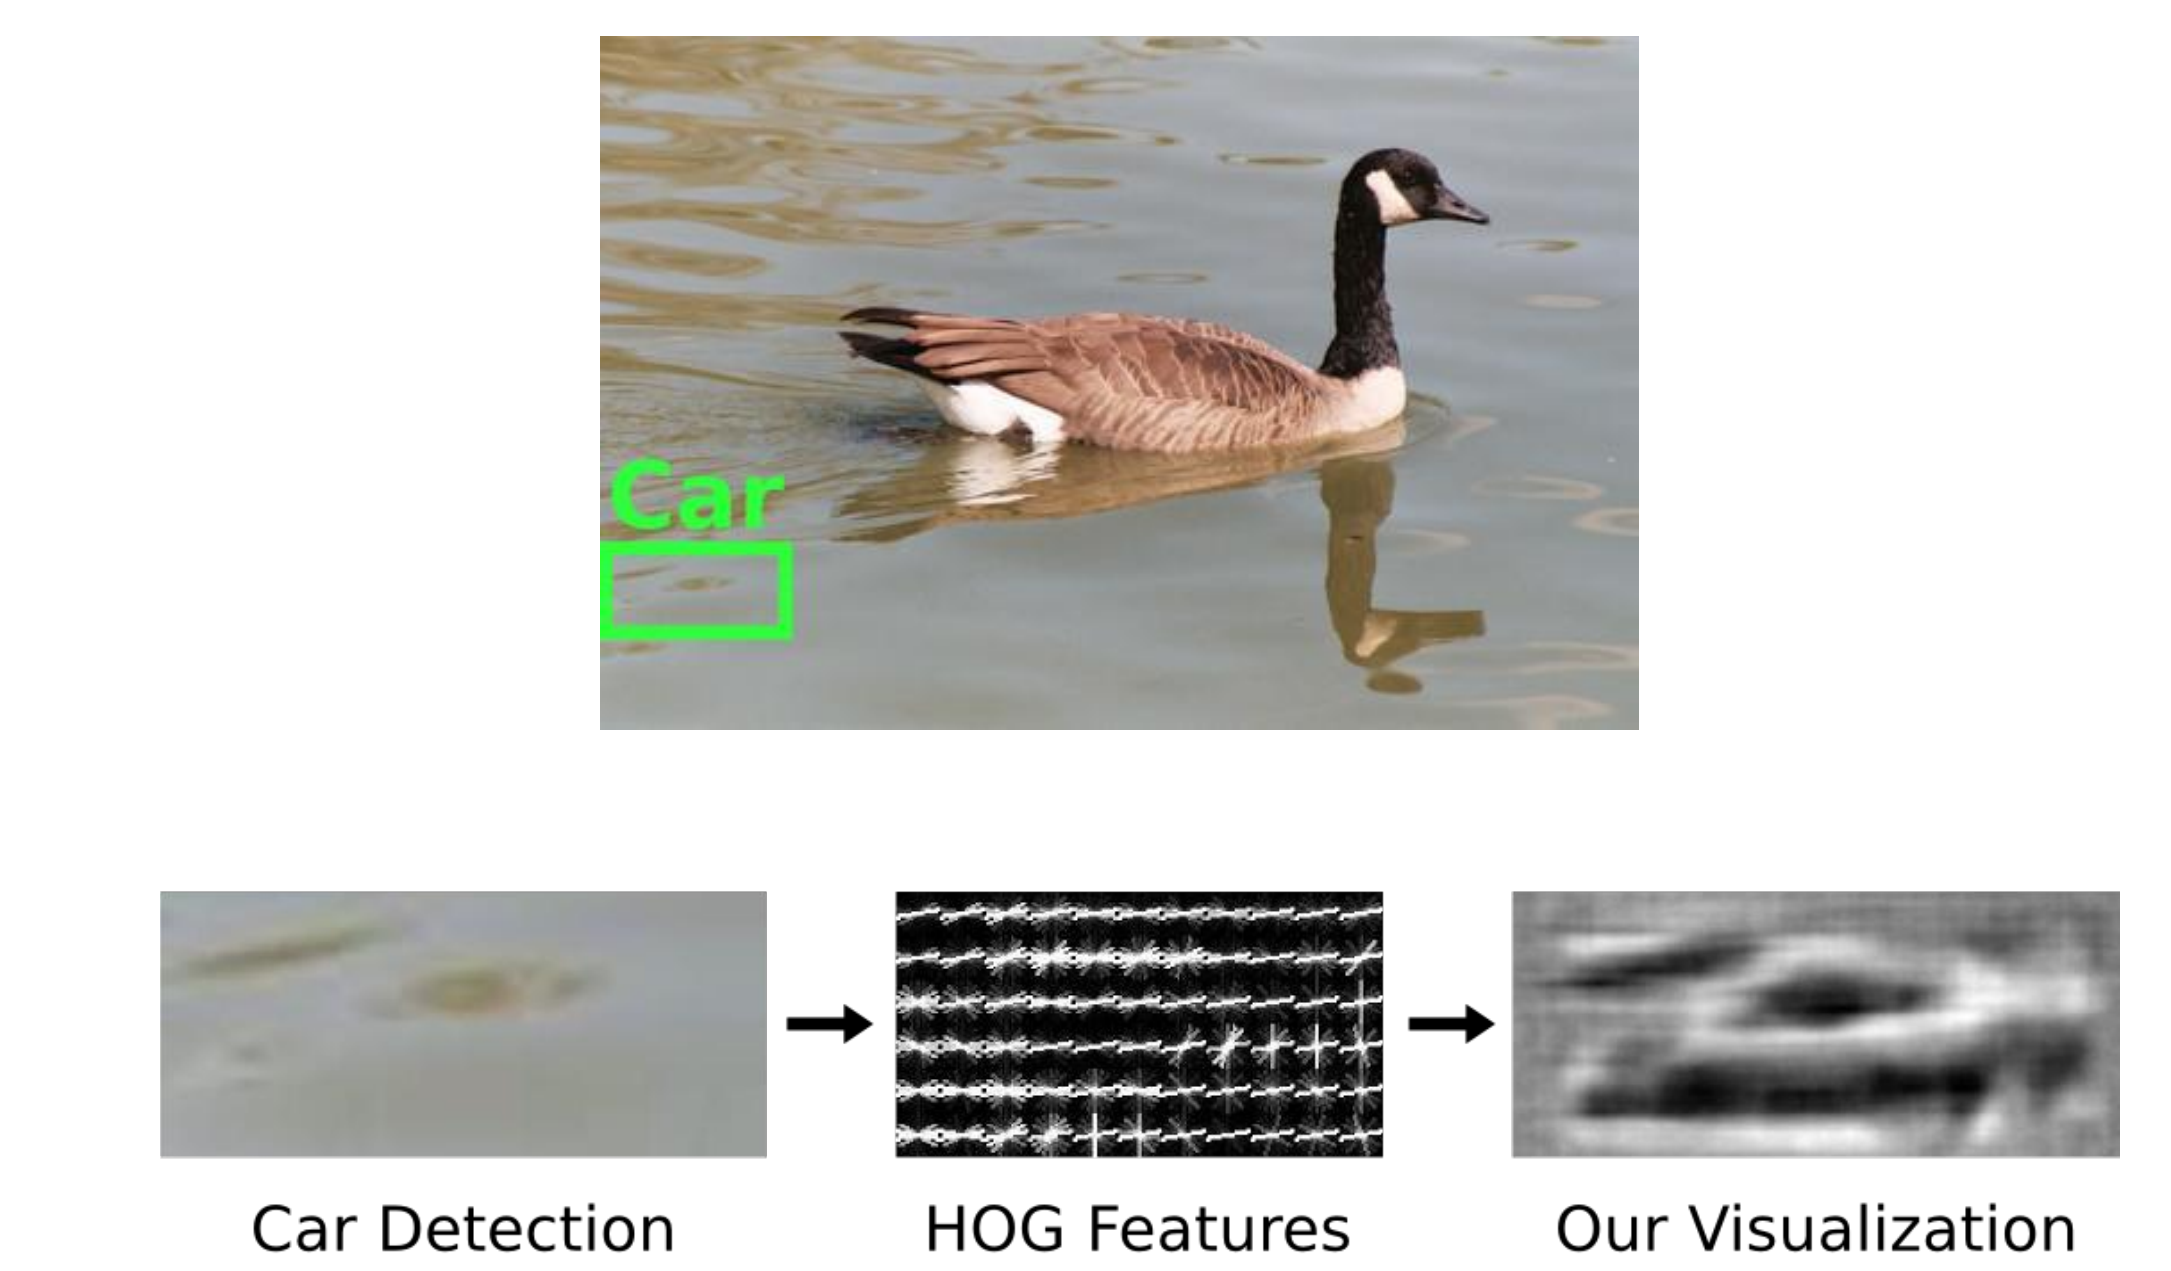
\includegraphics[width=0.6\linewidth]{img/HOGles}
\end{center}
